\documentclass[12pt]{article}
\usepackage{amsmath}
\usepackage{amsfonts}
\usepackage{graphicx}
\DeclareGraphicsExtensions{.pdf,.png,.jpg}

\newtheorem{theorem}{Theorem}[section]
\newtheorem{lemma}[theorem]{Lemma}
\newtheorem{definition}[theorem]{Definition}


\title{On Sampling}
\date{}
\begin{document}
  \maketitle
  
  \section{Continuous Sampling}
  Define $ball( x, r ) = \{ p \in \mathbb{R}: |p-x| \leq r \}$ as a ball in 1D. Consider sampling a 1D real line $L = [0, 1]$. Denote obstacles $O = \cup_{open intervals \in L}$, free space $F = \{ x \in L/O \}$. Let $S_{c} = \{ball(x,r) | \forall x \in L\}$. We define the sphere as a close sphere because we are using the upper bound of time for traveling from one configuration to another, the point on the boundary of a sphere is reachable. Let $C(S_{c})$ be the space covered by $S_{c}$. $C(S) = \cup_{b \in S}.$\\
  
  \subsection{Outer Sample}  
  Continuously sample spheres from left to right in the real line $L$, let the set of sphere be $S_{n}$, such that no sphere in $S_{n}$ is centered within any sphere of $S_{n}$. $S_{n} = \{ball(x)| \forall x_{i} \in \mathbb{R}, |x_{i} - x_{j}| \geq r_{j}, \forall j \neq i \}$.
  
  \begin{theorem}
  $C(S_{n}) = C(S_{c})$.
  \end{theorem}
  
  Proof:\\
  
  $\forall p \in L, \exists q=(p,r) \in S_{c}$, meaning every point in L is covered by one sphere centered at $x$ in $S_{c}$, $C(S_{c}) = L$. If sphere $q=(p,r)$ is not centered inside any spheres in $S_{n}$, then $q \in S_{n}$ and $p \in C(S_{n})$. Assume point $p$ is inside some existing spheres centered to the left of $p$, then $p \in C(S_{n})$. 
  
  To sum up, if point $p$ is sampled, then $p \in C(S_{c})$ and $p \in C(S_{n})$, if point $p$ is not sampled, still $p \in C(S_{c})$ and $p \in C(S_{n})$. Therefore, $C(S_{n}) = C(S_{c})$.\\
  
  ---------------------------------------------------------------------- \\
  
  This holds true also for 2D and 3D cases. If a point $p$ is sampled, then $p \in C(S_{n})$, if $p$ is not sampled, that is because it is already inside some existing spheres, so $p \in C(S_{n})$.
  
  Continuously sample points that are not inside any sphere is equivalent to continuously sample on the boundary of existing spheres.

  \begin{theorem}
  Sampling 1D real line $L$, $S_n$ is a finite set if the number of obstacles is finite.
  \end{theorem}
  
  Proof:
  
  Specify the real line to be a line segment $L = \{ x| 0 \leq x \leq 1 \}$, with obstacles in both ends. Start sampling from left to right, assume we are now sampling the i-th point $0 < x_i <= 0.25$, $q_i = (x_i, r_i), r_i = x_i$. Because $|x_{i} - x_{i-1}| < x_i = r_i$, $q_{i-1} \notin S_n$. If $0.25 < x_{i+1} < 0.5$, $S_n = \{ q_{i+1}, q_{i+2} \}$. If $x_{i+1} = 0.5$, $S_n = \{ q_{i+1} \}$. Every real line segment can be cut into finite number of smaller line segments with obstacles in both ends, if the number of obstacles is finite. Therefore $S_n$ is a finite set.
  
  \subsection{Minimum Radius Spheres}
  
  Let $S_m$ be a subset of $S_n$, such that no sphere in $S_m$ has radius less than $r_{min}$. $S_m = \{ q=(x,r) | \forall q \in S_n, r \geq r_{min} \}$  

  \begin{theorem}
  $S_m$ is a finite set.
  \end{theorem}

  Proof:\\

  Consider 2D case first.\\
  
  ( The idea is to find some iso-contours, where every point in a contour is equally far from obstacles, and sample on these contours. Then prove 3 things: 1. finite sample on a contour. 2. finite number of contours. 3. the sampled spheres set satisfies the definition of $S_m$ )  \\
  
  To prove this, we need some medium conclusions: \\
  
  1. Let $\lambda$ be a finite path in 2D world, $S_p = \{ q = {x,r} | \forall x \in \lambda, r = C \}$, where $C$ is a constant. $S_p$ is a finite set. This is because every sphere with fixed radius will cover at least $2 \cdot C$ length of the path, as long as the path is finite, the number of spheres sampled in the path will not be infinite.\\
  
  2. ( By choosing the distance between each contour, the number of contours is finite, because we have minimum distance from obstacles and upper bound distance from obstacles. )\\
  
  3. ( Assume we have some initial contours, say voronoi graph edges, and we sample spheres on the contour, if we choose the new contours to be 1/2 distance from obstacles to the existing contours, then sample on the new contour. Repeat the process until converge( the new contour is exactly $r_{min}$ away from obstacles). ).\\
  
  PS:\\
  
  Sampling on media axis can be done without computing axis first. Read: MAPRM: A Probabilistic Roadmap Planner with Sampling on the Medial Axis of the Free Space, Steven A. Wilmarth, Nancy M. Amato, Peter F. Stiller, In Proc. IEEE Int. Conf. Robot. Autom. (ICRA), pp. 1024-1031, Detroit, MI, May 1999. Also, Technical Report, TR98-0022, Department of Computer Science and Engineering, Texas A&M University, Nov 1998. 
  
==============================================================================

==============================================================================  

==============================================================================\\  
  %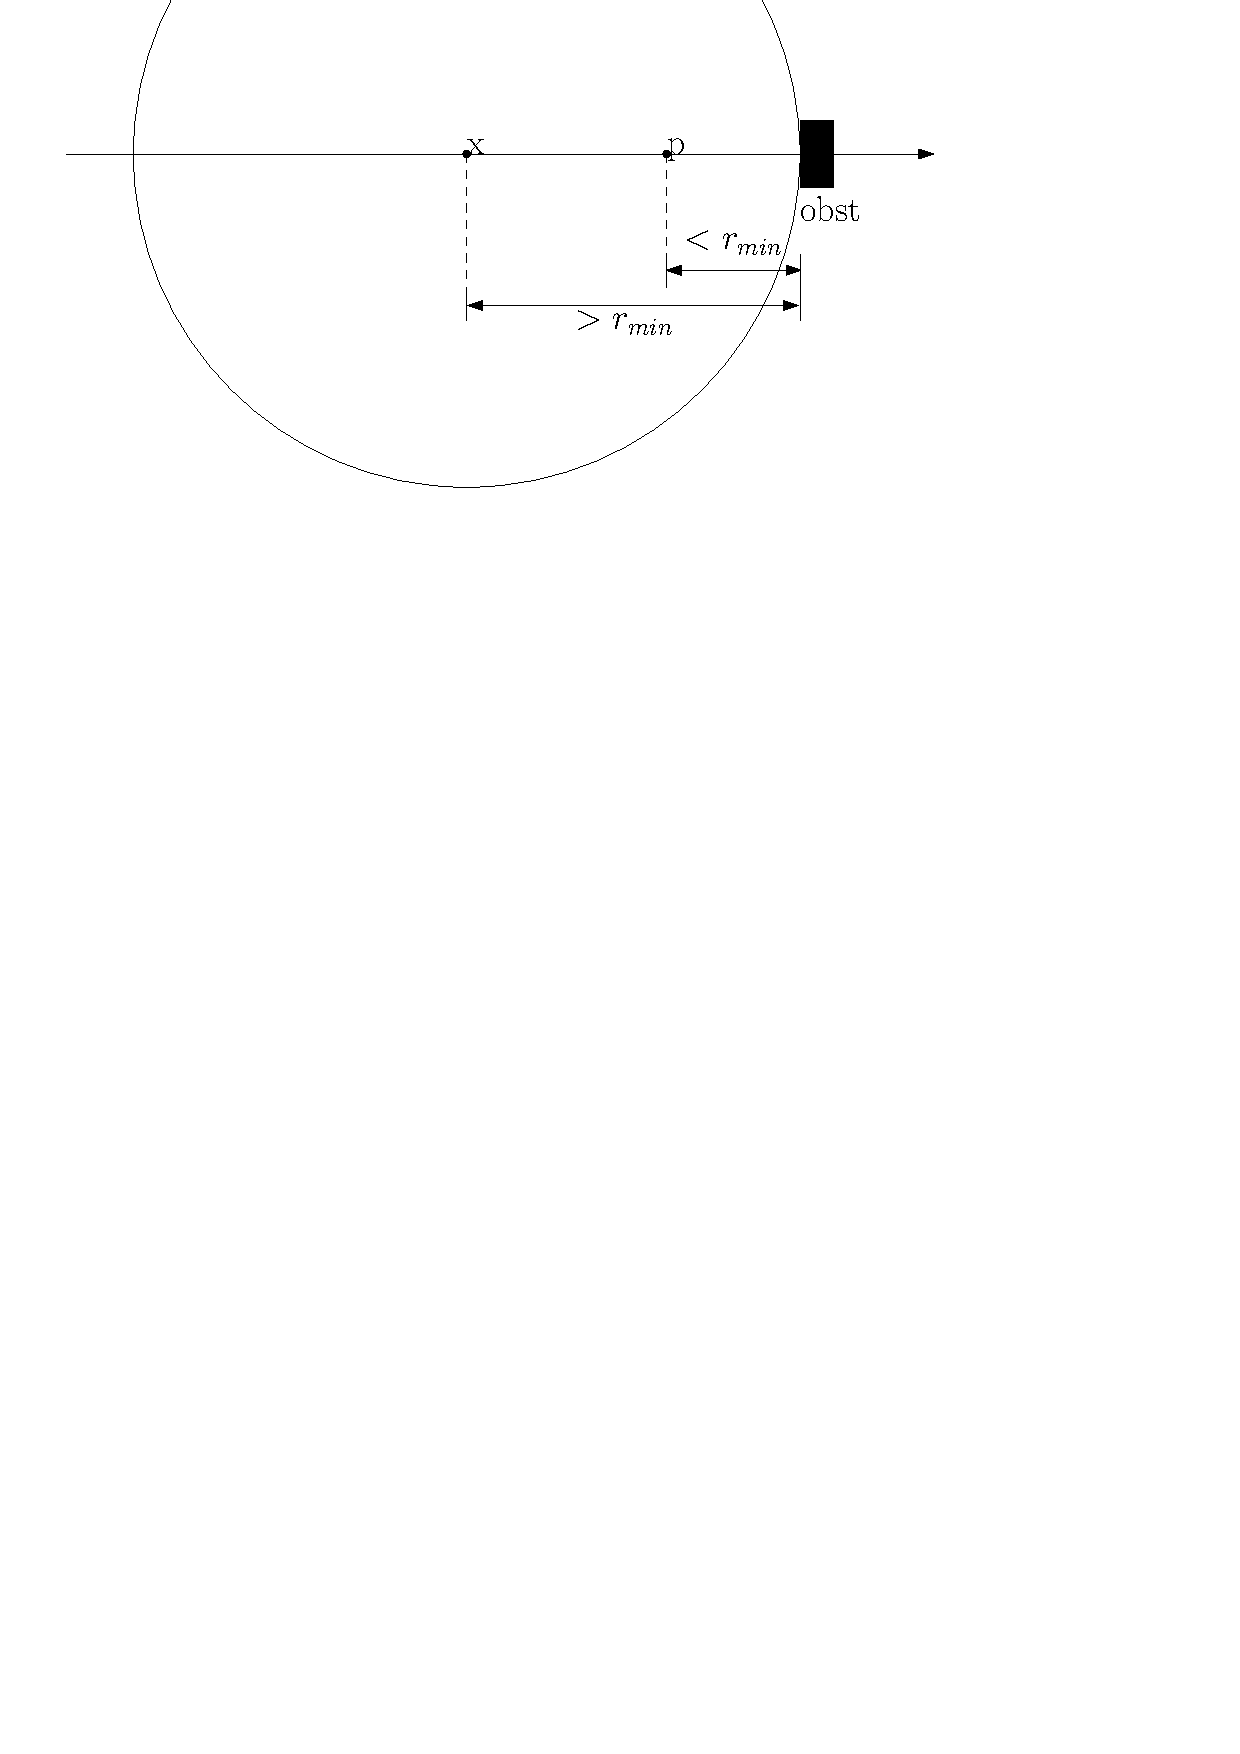
\includegraphics[scale=0.8]{sample_S_m}  
  
  %---------------------------------------------------------------------- \\
  
  %For 2D and 3D this is different:\\
  
  %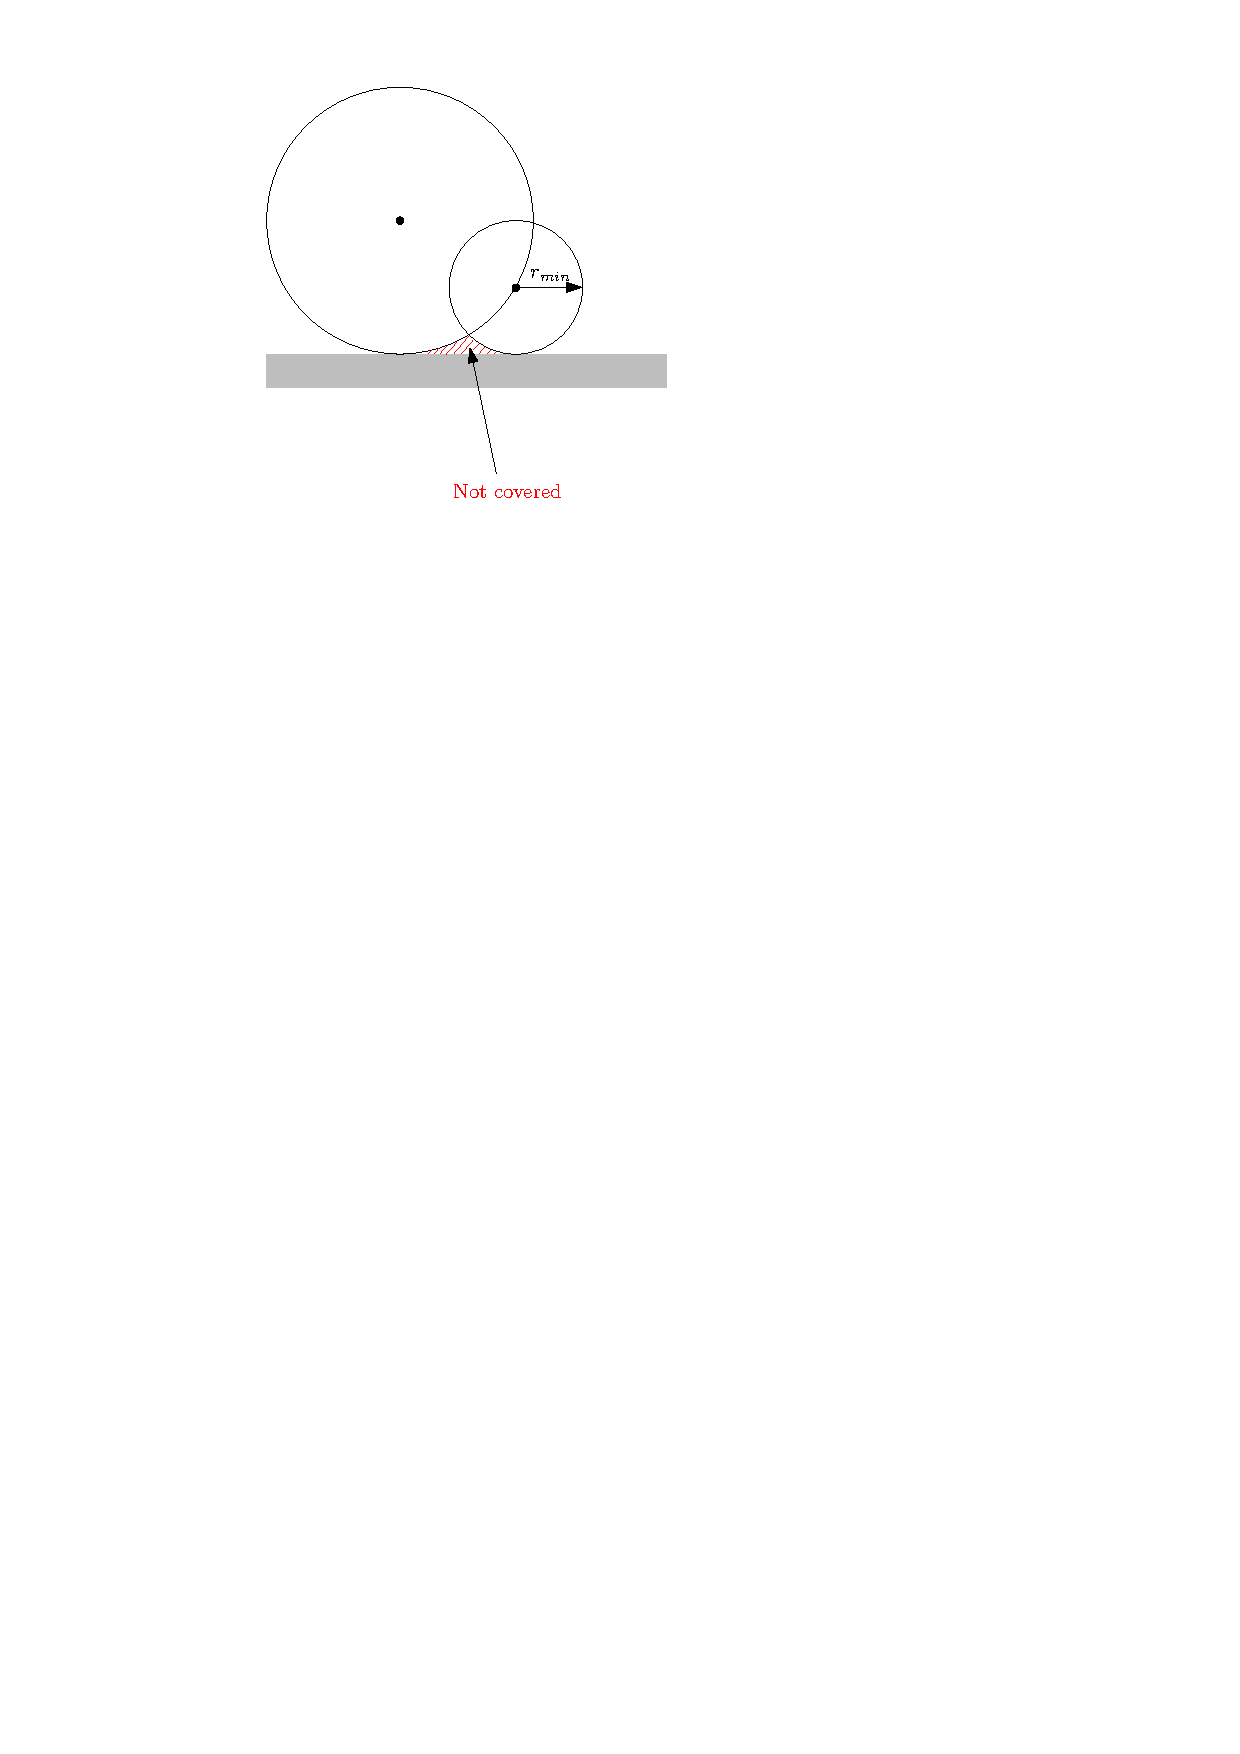
\includegraphics[scale=0.8]{sample2D_S_m}  \\
  
  %A possible way to reduce the uncovered area is to more densely sample areas close to obstacles. For example, allow spheres to center inside existing spheres in this area.
  
  \subsection{Inaccurate Metric}
  Sample spheres continuously in the space such that no sphere is inside existing ones and all spheres have radius more than $r_{min}$. Assume the sampling metric gives 1/n of the real distance to obstacles. Denote the set of spheres as $S_{in}$.
  \begin{theorem}
  Any point $p$ within $(n-1) \cdot r_{min}$ distance away from obstacles, $p \notin C(S_(in))$.
  \end{theorem}
  
  Proof:\\
  
  Assume $p$ is $(n-1) \cdot r_{min}$ distance away from obstacles, if there exists point $x$ that is $n \cdot r_{min}$ distance away from obstacles, then sphere $q_{x}$ has radius $r_{min}$, $p \in q_{x}$. 
  
  If $p$ is $(n-1) \cdot r_{min} - \epsilon$ distance away from obstacles, where $\epsilon >= 0$, we need a point $x$ that is within $n \cdot r_{min} - \frac{n \cdot \epsilon}{n-1}$ distance from obstacle.  The sphere sampled at $x$ has radius less than $r_{min}$ thus will not cover point p.\\
 
  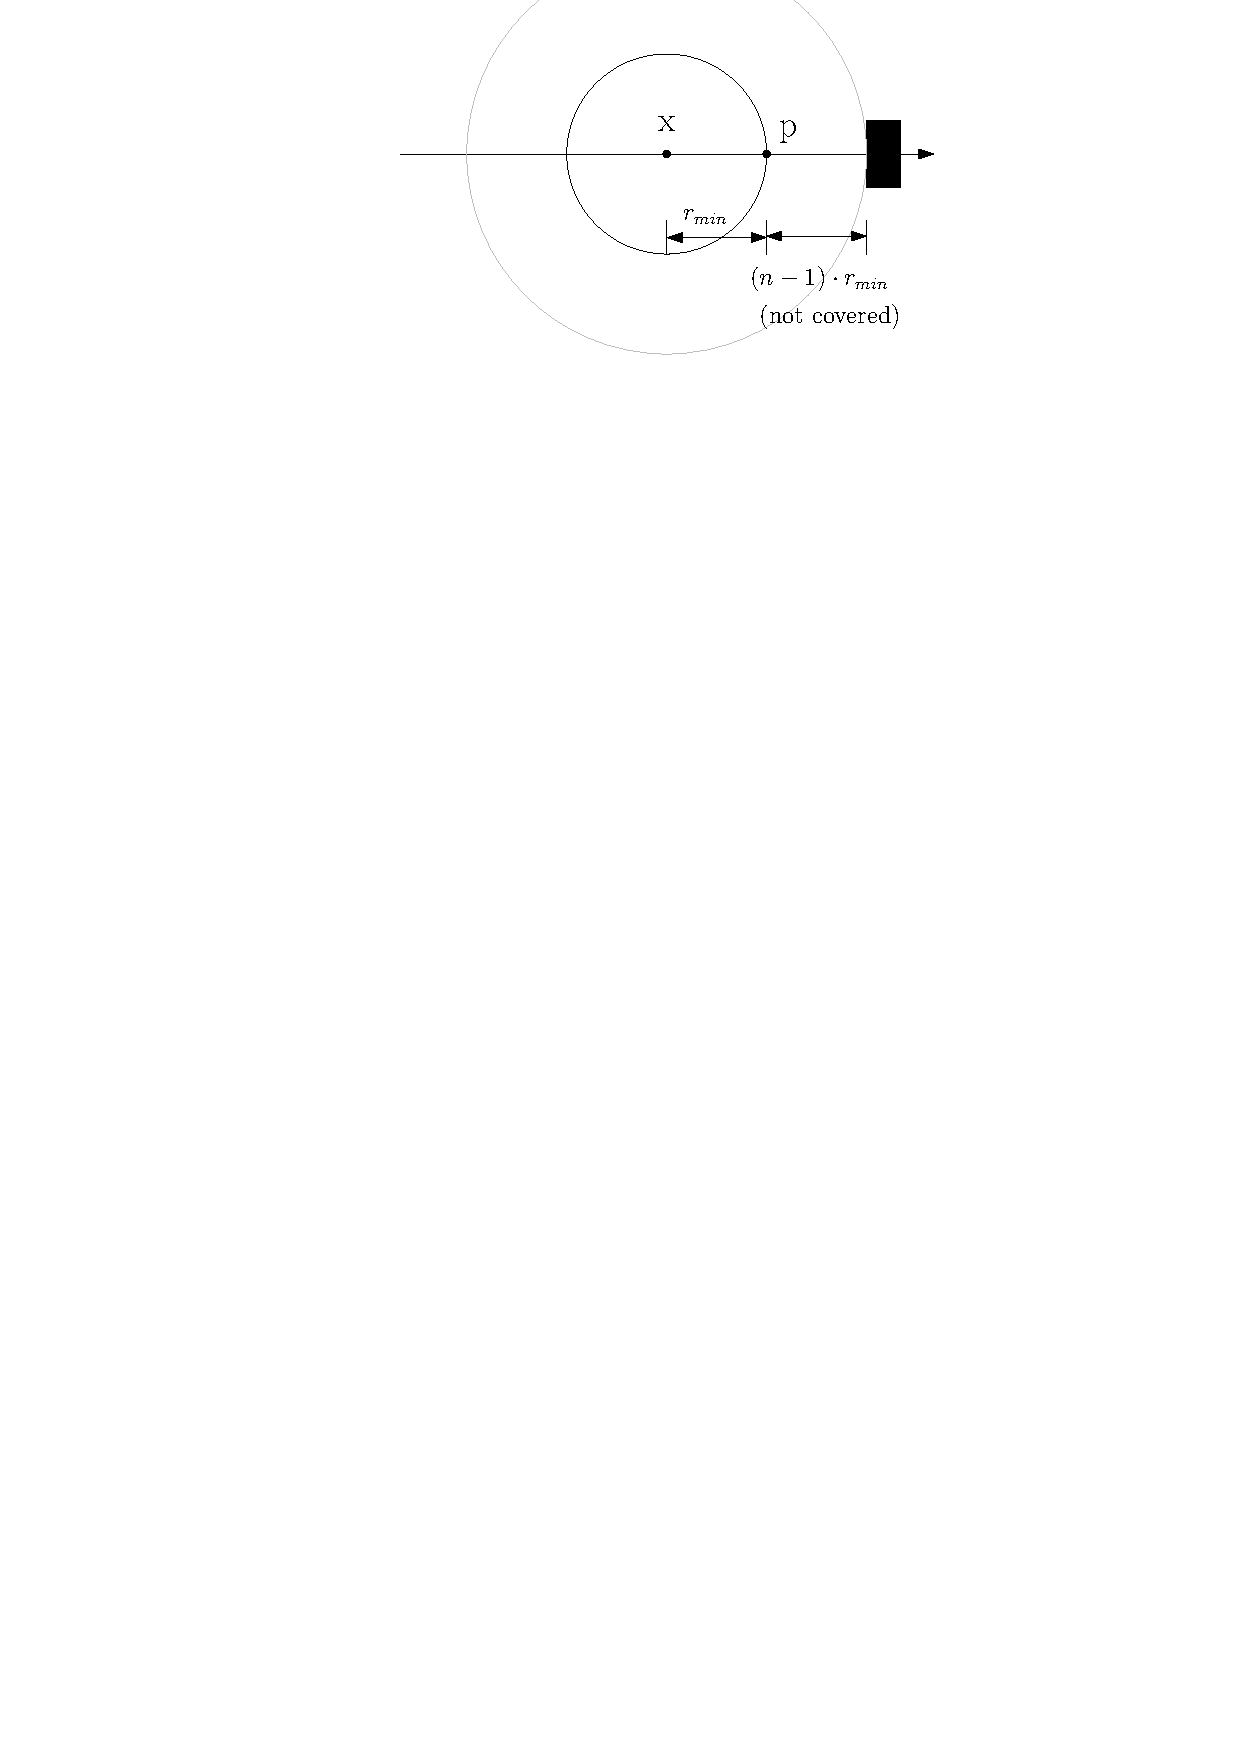
\includegraphics[scale=0.8]{sample_S_in} \\
  
  --------------------------------------------------------------------\\
  
  This is also true for 2D and 3D cases. Introduce a line from the closest point in obstacle in normal direction, then the proof is the same. However, uncovered area as shown in Theorem 1.2 stays still.
  
  \begin{theorem}
  Let $S_{d}$ be a subset of $S_{in}$ by discrete sampling in the real line. Assume every two neighbor samples are $d$ distance away from each other. If $d <= \frac{r_{min}}{k}, k>=1$, in the worst case, any point $p$ that has clearance less than $\frac{r_{min} \cdot (n-1)}{k \cdot n} + (n-1) \cdot r_{min}$, $p \notin C(S_d)$.
  \end{theorem}
  
  As is shown in last theorem, the smallest clearance a point $x$ should have in order to be sampled is $n \cdot r_{min}$. $\exists \epsilon > 0$, point $x_{t}$ with clearance $n \cdot r_{min} + d - \epsilon$. The point the sphere $q_{x_{t}}$ can cover has clearance more than  $(n-1) \cdot r_{min} + \frac{d \cdot (n-1)}{n} - \frac{(n-1) \cdot \epsilon}{n}$. The worst case is $\epsilon = 0$, so the clearance is $(n-1) \cdot r_{min} + \frac{d \cdot (n-1)}{n} = (n-1) \cdot r_{min} + \frac{r_{min} \cdot (n-1)}{k \cdot n}$
    
  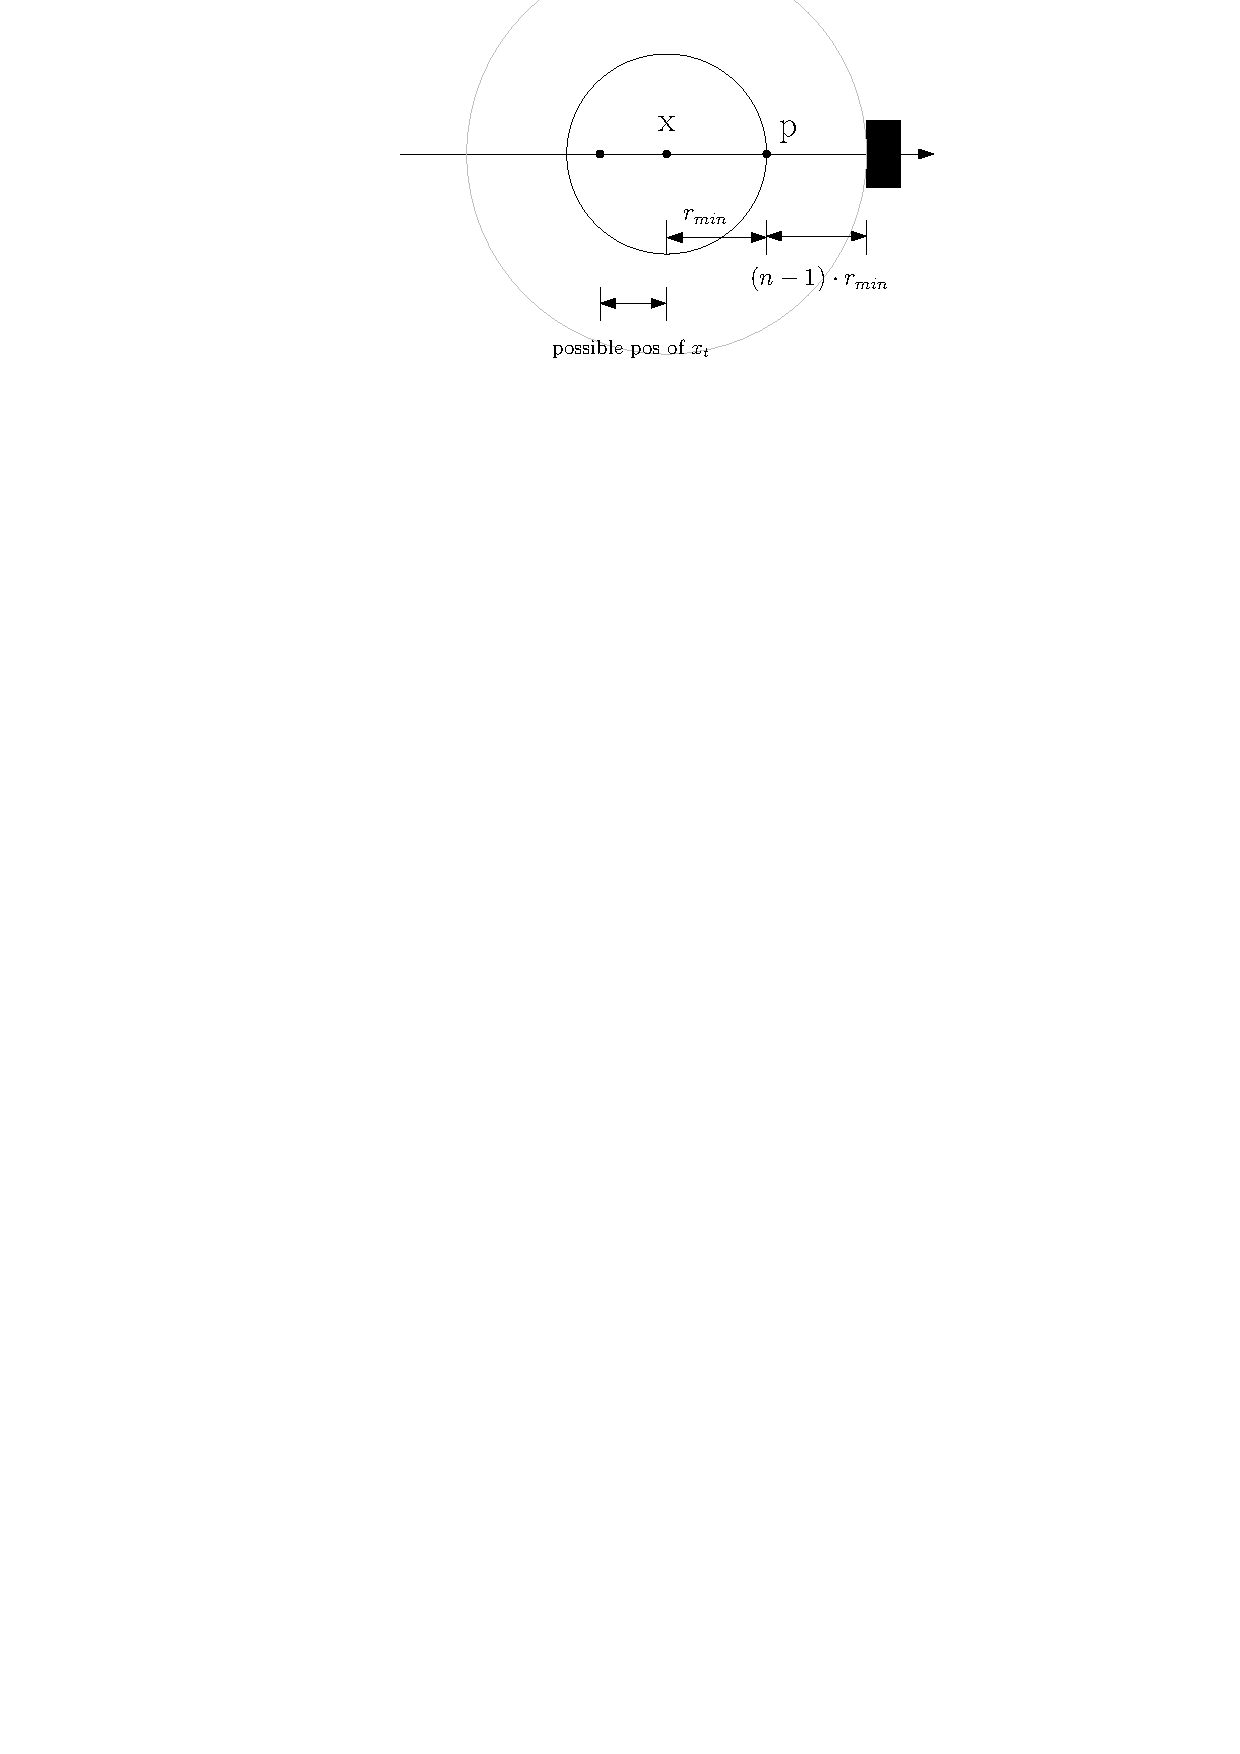
\includegraphics[scale=0.8]{sample_S_d}\\
  
  --------------------------------------------------------------------\\  
  
  In 2D the possible position for $x_{t}$ is a square, it will be a cube in 3D, the result is very similar except for that the uncovered area introduced by Theorem 1.2 is still can't be removed.\\

  
==============================================================================

==============================================================================  

==============================================================================\\
  
      
\end{document}
  